\documentclass[sigconf,
review,
anonymous,
%draft,
%authorversion,
screen
]{acmart}

\usepackage{booktabs} % For formal tables
%\usepackage{balance}

\usepackage{pgfplots}
\usepackage{tikzscale}
\pgfplotsset{compat=newest}

% ----------------------
% fancyref
\usepackage[plain]{fancyref}

\newcommand*{\fancyrefalglabelprefix}{alg}
\newcommand*{\fancyreflstlabelprefix}{lst}
\newcommand*{\fancyrefapplabelprefix}{app}

\fancyrefaddcaptions{english}{%
	\providecommand*{\frefalgname}{algorithm}%
	\providecommand*{\Frefalgname}{Algorithm}%
	%
	\providecommand*{\freflstname}{listing}%
	\providecommand*{\Freflstname}{Listing}%
	%
	\providecommand*{\frefappname}{appendix}%
	\providecommand*{\Frefappname}{Appendix}%
}%

\frefformat{plain}{\fancyrefalglabelprefix}{%
	\frefalgname\fancyrefdefaultspacing#1%
}%
\Frefformat{plain}{\fancyrefalglabelprefix}{%
	\Frefalgname\fancyrefdefaultspacing#1%
}
\frefformat{vario}{\fancyrefalglabelprefix}{%
	\frefalgname\fancyrefdefaultspacing#1#3%
}%
\Frefformat{vario}{\fancyrefalglabelprefix}{%
	\Frefalgname\fancyrefdefaultspacing#1#3%
}%

\frefformat{plain}{\fancyreflstlabelprefix}{%
	\freflstname\fancyrefdefaultspacing#1%
}%
\Frefformat{plain}{\fancyreflstlabelprefix}{%
	\Freflstname\fancyrefdefaultspacing#1%
}
\frefformat{vario}{\fancyreflstlabelprefix}{%
	\freflstname\fancyrefdefaultspacing#1#3%
}%
\Frefformat{vario}{\fancyreflstlabelprefix}{%
	\Freflstname\fancyrefdefaultspacing#1#3%
}%

\frefformat{plain}{\fancyrefapplabelprefix}{%
	\frefappname\fancyrefdefaultspacing#1%
}%
\Frefformat{plain}{\fancyrefapplabelprefix}{%
	\Frefappname\fancyrefdefaultspacing#1%
}
\frefformat{vario}{\fancyrefapplabelprefix}{%
	\frefappname\fancyrefdefaultspacing#1#3%
}%
\Frefformat{vario}{\fancyrefapplabelprefix}{%
	\Frefappname\fancyrefdefaultspacing#1#3%
}%



\newcommand{\dummyfig}[3]{
	\centering
	\fbox{
		\begin{minipage}[c][#1\textheight][c]{#2\textwidth}
			\centering{#3}
		\end{minipage}
	}
}


% Copyright
%\setcopyright{none}
%\setcopyright{acmcopyright}
%\setcopyright{acmlicensed}
%\setcopyright{rightsretained}
%\setcopyright{usgov}
%\setcopyright{usgovmixed}
%\setcopyright{cagov}
%\setcopyright{cagovmixed}
\copyrightyear{2018} 
\acmYear{2018} 
\setcopyright{acmcopyright}

% DOI
%\acmDOI{10.475/123_4}

% ISBN
%\acmISBN{123-4567-24-567/08/06}

%Conference
\acmConference[BigVis'18]{International Workshop on Big Data Visual Exploration and Analytics at EDBT/ICDT}{March 2018}{Vienna, Austria} 

%\acmYear{1997}
%\copyrightyear{2016}


%\acmArticle{4}
\acmPrice{00.00}

% These commands are optional
%\acmBooktitle{Transactions of the ACM Woodstock conference}
%\editor{Jennifer B. Sartor}
%\editor{Theo D'Hondt}
%\editor{Wolfgang De Meuter}


\begin{document}
\title%
[Topic-aware Network Visualisation]%
{Topic-aware Network Visualisation to\\Explore Large Email Corpora}
%\titlenote{Produces the permission block, and copyright information}
%\subtitle{Extended Abstract}
%\subtitlenote{The full version of the author's guide is available as \texttt{acmart.pdf} document}


\author{Tim Repke}
\affiliation{%
  \institution{Hasso Plattner Institute}
  \city{Potsdam} 
  \country{Germany}
}
\email{tim.repke@hpi.de}
\author{Ralf Krestel}
\affiliation{%
	\institution{Hasso Plattner Institute}
	\city{Potsdam} 
	\country{Germany}
}
\email{ralf.krestel@hpi.de}

% The default list of authors is too long for headers.
\renewcommand{\shortauthors}{T. Repke and R. Krestel}


\begin{abstract}

Nowadays, more and more large datasets exhibit an intrinsic graph structure.
While there exist special graph databases to handle ever increasing amounts of nodes and edges, visualising this data becomes infeasible quickly with growing data.
In addition, looking at its structure is not sufficient to get an overview of a graph dataset.
Indeed, visualising additional information about nodes or edges without cluttering the screen is essential.
In this paper, we propose an interactive visualisation for social networks that positions individuals (nodes) on a two-dimensional canvas such that communities defined by social links (edges) are easily recognisable.
Furthermore, we visualise topical relatedness between individuals by analysing information about social links, in our case email communication.
To this end, we utilise document embeddings, which project the content of an email message into a high dimensional
semantic space and graph embeddings, which project nodes in a network graph into a latent space reflecting their relatedness.

\end{abstract}

%
% The code below should be generated by the tool at
% http://dl.acm.org/ccs.cfm
% Please copy and paste the code instead of the example below. 
%
%\begin{CCSXML}
%<ccs2012>
% <concept>
%  <concept_id>10010520.10010553.10010562</concept_id>
%  <concept_desc>Computer systems organization~Embedded systems</concept_desc>
%  <concept_significance>500</concept_significance>
% </concept>
% <concept>
%  <concept_id>10010520.10010575.10010755</concept_id>
%  <concept_desc>Computer systems organization~Redundancy</concept_desc>
%  <concept_significance>300</concept_significance>
% </concept>
% <concept>
%  <concept_id>10010520.10010553.10010554</concept_id>
%  <concept_desc>Computer systems organization~Robotics</concept_desc>
%  <concept_significance>100</concept_significance>
% </concept>
% <concept>
%  <concept_id>10003033.10003083.10003095</concept_id>
%  <concept_desc>Networks~Network reliability</concept_desc>
%  <concept_significance>100</concept_significance>
% </concept>
%</ccs2012>  
%\end{CCSXML}
%
%\ccsdesc[500]{Computer systems organization~Embedded systems}
%\ccsdesc[300]{Computer systems organization~Redundancy}
%\ccsdesc{Computer systems organization~Robotics}
%\ccsdesc[100]{Networks~Network reliability}
%
%
%\keywords{ACM proceedings, \LaTeX, text tagging}

% Deadline 26.12.2017 02:00am
%\received{December 2017}
%\received[revised]{January 2018}
%\received[accepted]{January 2018}

\settopmatter{printccs=false, printacmref=false, printfolios=true}

\maketitle

\section{Introduction}
% abstract + intro fill first page

% information society, modern, communication, integral part of daily life, substantial amounts of data, prior research either topics or networks (not both)

In our modern information society, we produce substantial amounts of data each day, where a large portion of it comes from the communication through social media platforms or email.
Given a dataset of the exchanged information over a year or more, it is practically impossible to gain an overview or quick insights into the data.
Journalists, for example, find themselves in this position whenever they receive huge collections of leaked data.
A system that automatically generates an overview of latent structures and topics may support the exploratory search for potential stories and related documents as well as a basic understanding of the data.

In this paper, we propose an interactive visualisation that positions individuals on a two-dimensional canvas such that it reflects their community in which they communicate along with their the topical relatedness.
Therefore, we utilise document embeddings which project the content of a message into a high dimensional semantic space and graph embeddings, which project nodes in a network graph into a latent space reflecting their relatedness.

The proposed system is best described as an exploratory search engine.
As such, it is well suited for users unfamiliar with the domain and terminology in the collection at hand and they can iteratively discover new associations to support the information seeking process of an open-ended goal~\cite{white2009exploratory}.
% p9: exploratory strategies are used continually to allow people to discover new associations, kinds of knowledge, and decision making, they are often motivated by a complex information problem, a poor understanding of terminology and information space structure
% p10: people engaged in exploratory searches are generally: (1) unfamiliar with the domain of their goal (i.e., need to learn about the topic in order to understand how to achieve their goal);
% p10: Exploratory search is a specialization of information seeking, which describes the activity of attempting to obtain information through a combination of querying and collection browsing.
In particular, we focus on visualising the entire collection in one overview in which related aspects are spatially close and therefore reflecting a latent context.
To our knowledge, prior research only considers either network or text visualisation.
We aim to combine these two approaches so that it can be applied to document collections with an underlying network, such as an email corpus.
For that goal, we consider the concept of map-like visualisations~\cite{pang2017creating}, which was previously used for both network and text data.

There are various objectives for network visualisations.
For example, ContactTrees~\cite{sallaberry2016contact} makes use of the metaphor of a growing tree to show highlight how relationships form and change based on the interactions as branches and leaves.
Although this reflects temporal aspects of dynamic networks well, it focuses on one person as the root, thus an overview of the entirety of a network is lost.
A CactusTree~\cite{dang2017cactustree} on the other hand is a technique to represent hierarchical structures with the goal of untangling overlaid bundles of intersecting edges, making distant connections more apparent.
In networks with evolving relations, higher order dependencies may get lost in traditional visualisations.
HoNVis~\cite{tao2017honvis} adds nodes to encode dependencies in chains of interactions similar to conditional probabilities.
Usually though, a communication network has many nodes and overlapping connections already, so Yang et al.~\cite{yang2014overlapping} rather focus on discovering overlapping cores in the network to improve the identification of community boundaries, providing an overview of global latent structures.
Similarly, Gronemann et al.~\cite{gronemann2012drawing} use the metaphor of islands and hills to visualise clustered graphs, making densely connected communities clearly noticeable.
The edges are bundled and follow valleys of the resulting topology, thus making relationships between other communities hard to follow.
MapSets~\cite{efrat2015mapsets} assume a graph that was laid out using embeddings reflecting communities.
An algorithm then draws regions around clusters of nodes, such that the bounding shapes are contiguous and non-overlapping, but yet abstract.
Another approach to visualise networks at full scale is to aggregate nodes based on their spatial distribution and thereby allowing for a simple exploration as proposed by Hildenbrand et al.~\cite{hildenbrand2016flexible}, who also added contour lines and heatmap overlays to emphasise latent structures.

% ==== GRAPH VIS ====
%\cite{dang2017cactustree}
%visualization technique for representing hierarchical datasets, specific goal of untangling overlaid bundles of intersecting edges.
%\cite{sallaberry2016contact}
%highlight how relationships form and change based upon interactions among actors, as well as how relationships and networks vary by contact attributes
%
%\cite{tao2017honvis}
%higher order visualisation of network by adding (splitting) nodes to encode higher-order dependencies (ie conditional probability), Objective: (ie) discover ports relevant for species invasion, extract higher order dependencies (ie not pairwise, but tuple of len 3 -> cond prob of last node given first node)
%\cite{yang2014overlapping}
%discover overlapping "cores" in network graph for more accurate communities and improved identification of community boundaries
%
%\cite{gronemann2012drawing}
%clustered graph as map with islands
%\cite{efrat2015mapsets}
%visualising embedded+clustered graphs, find regions, how to map them out nicely
%\cite{hildenbrand2016flexible}
%aggregates nodes based on their spatial distribution, thereby allowing for visual exploration of large graphs, contour lines/heatmap

Document visualisation aims to visualise the content, such that users gain quick insights into topics, latent phrases, or trends.
Tiara~\cite{wei2010tiara} extracts topics and derives time-sensitive keywords to depict evolving subjects over time as stacked plots.
Other approaches often project documents into a latent space, either using topic models or embeddings.
Creating scatter-plots of embedded documents of a large corpus may result in a very dense and unclear layout, so Chen et al.~\cite{chen2009exemplar} developed an algorithm to reduce over-full visualisations by picking representative documents.
A different approach is taken by Fortuna et al.~\cite{fortuna2005visualization}, who don't show documents directly, but generate a heatmap of the populated canvas and overlay it with salient phrases at more densely populated areas from the underlying documents in that region.
Friedl et al.~\cite{fried2014maps} extend that concept by drawing clear lines drawing clear lines between regions and colouring them.
They also add edges between salient phrases based on co-occurrences in the texts and adjusting their size reflecting the count.
Most recently Cartograph~\cite{sen2017cartograph} was proposed, which is visually very similar to previous approaches, but uses pre-rendered information of different resolution and map technology to enable a responsive interactive visualisation. Regions are coloured based on underlying ontologies from a knowledge-base.

% === TEXT VIS ===
%\cite{wei2010tiara}
%Extract topics and derive time-sensitive keywords to depict the content evolution of each topic over time visualised as stacked plots
%\cite{chen2009exemplar}
%pick exemplars to reduce over-full visualisation (scatter plot)
%\cite{fortuna2005visualization}
%visualise text corpus (heatmaps + dots for docs + salient phrases)
%\cite{fried2014maps}
%maps of computer science, similar but draws clear regions and edges reflecting co-occurrence
%\cite{sen2017cartograph}
%Visualisation System for thematic maps that position Concepts (ie Named Entities) into semantic space on map, pre-render and use maps technology

% 
%\cite{wang2016linked}
%which combines link and label information with content information to learn document representations for classification
%\cite{goyal2017graph}
%graph embedding survey
%\cite{bikakis2016exploration}
% visual exploration of big liked semantic data - challenges


%related work
%\begin{itemize}
%	\item two parts: network vis, textvis
%	\item embeddings: doc2vec, node2vec
%	\item hierarchical/level of detail
%	\item map semantic
%	\item cartograph close to us, but no network
%	\item highlight missing link between text and network in all research
%\end{itemize}

%introduce topic, challenges, rough goal, related work

\begin{figure*}
	%	\centering
	\begin{tikzpicture}[]
	\node[draw,anchor=north west,inner sep=1] at (0,0) {%
		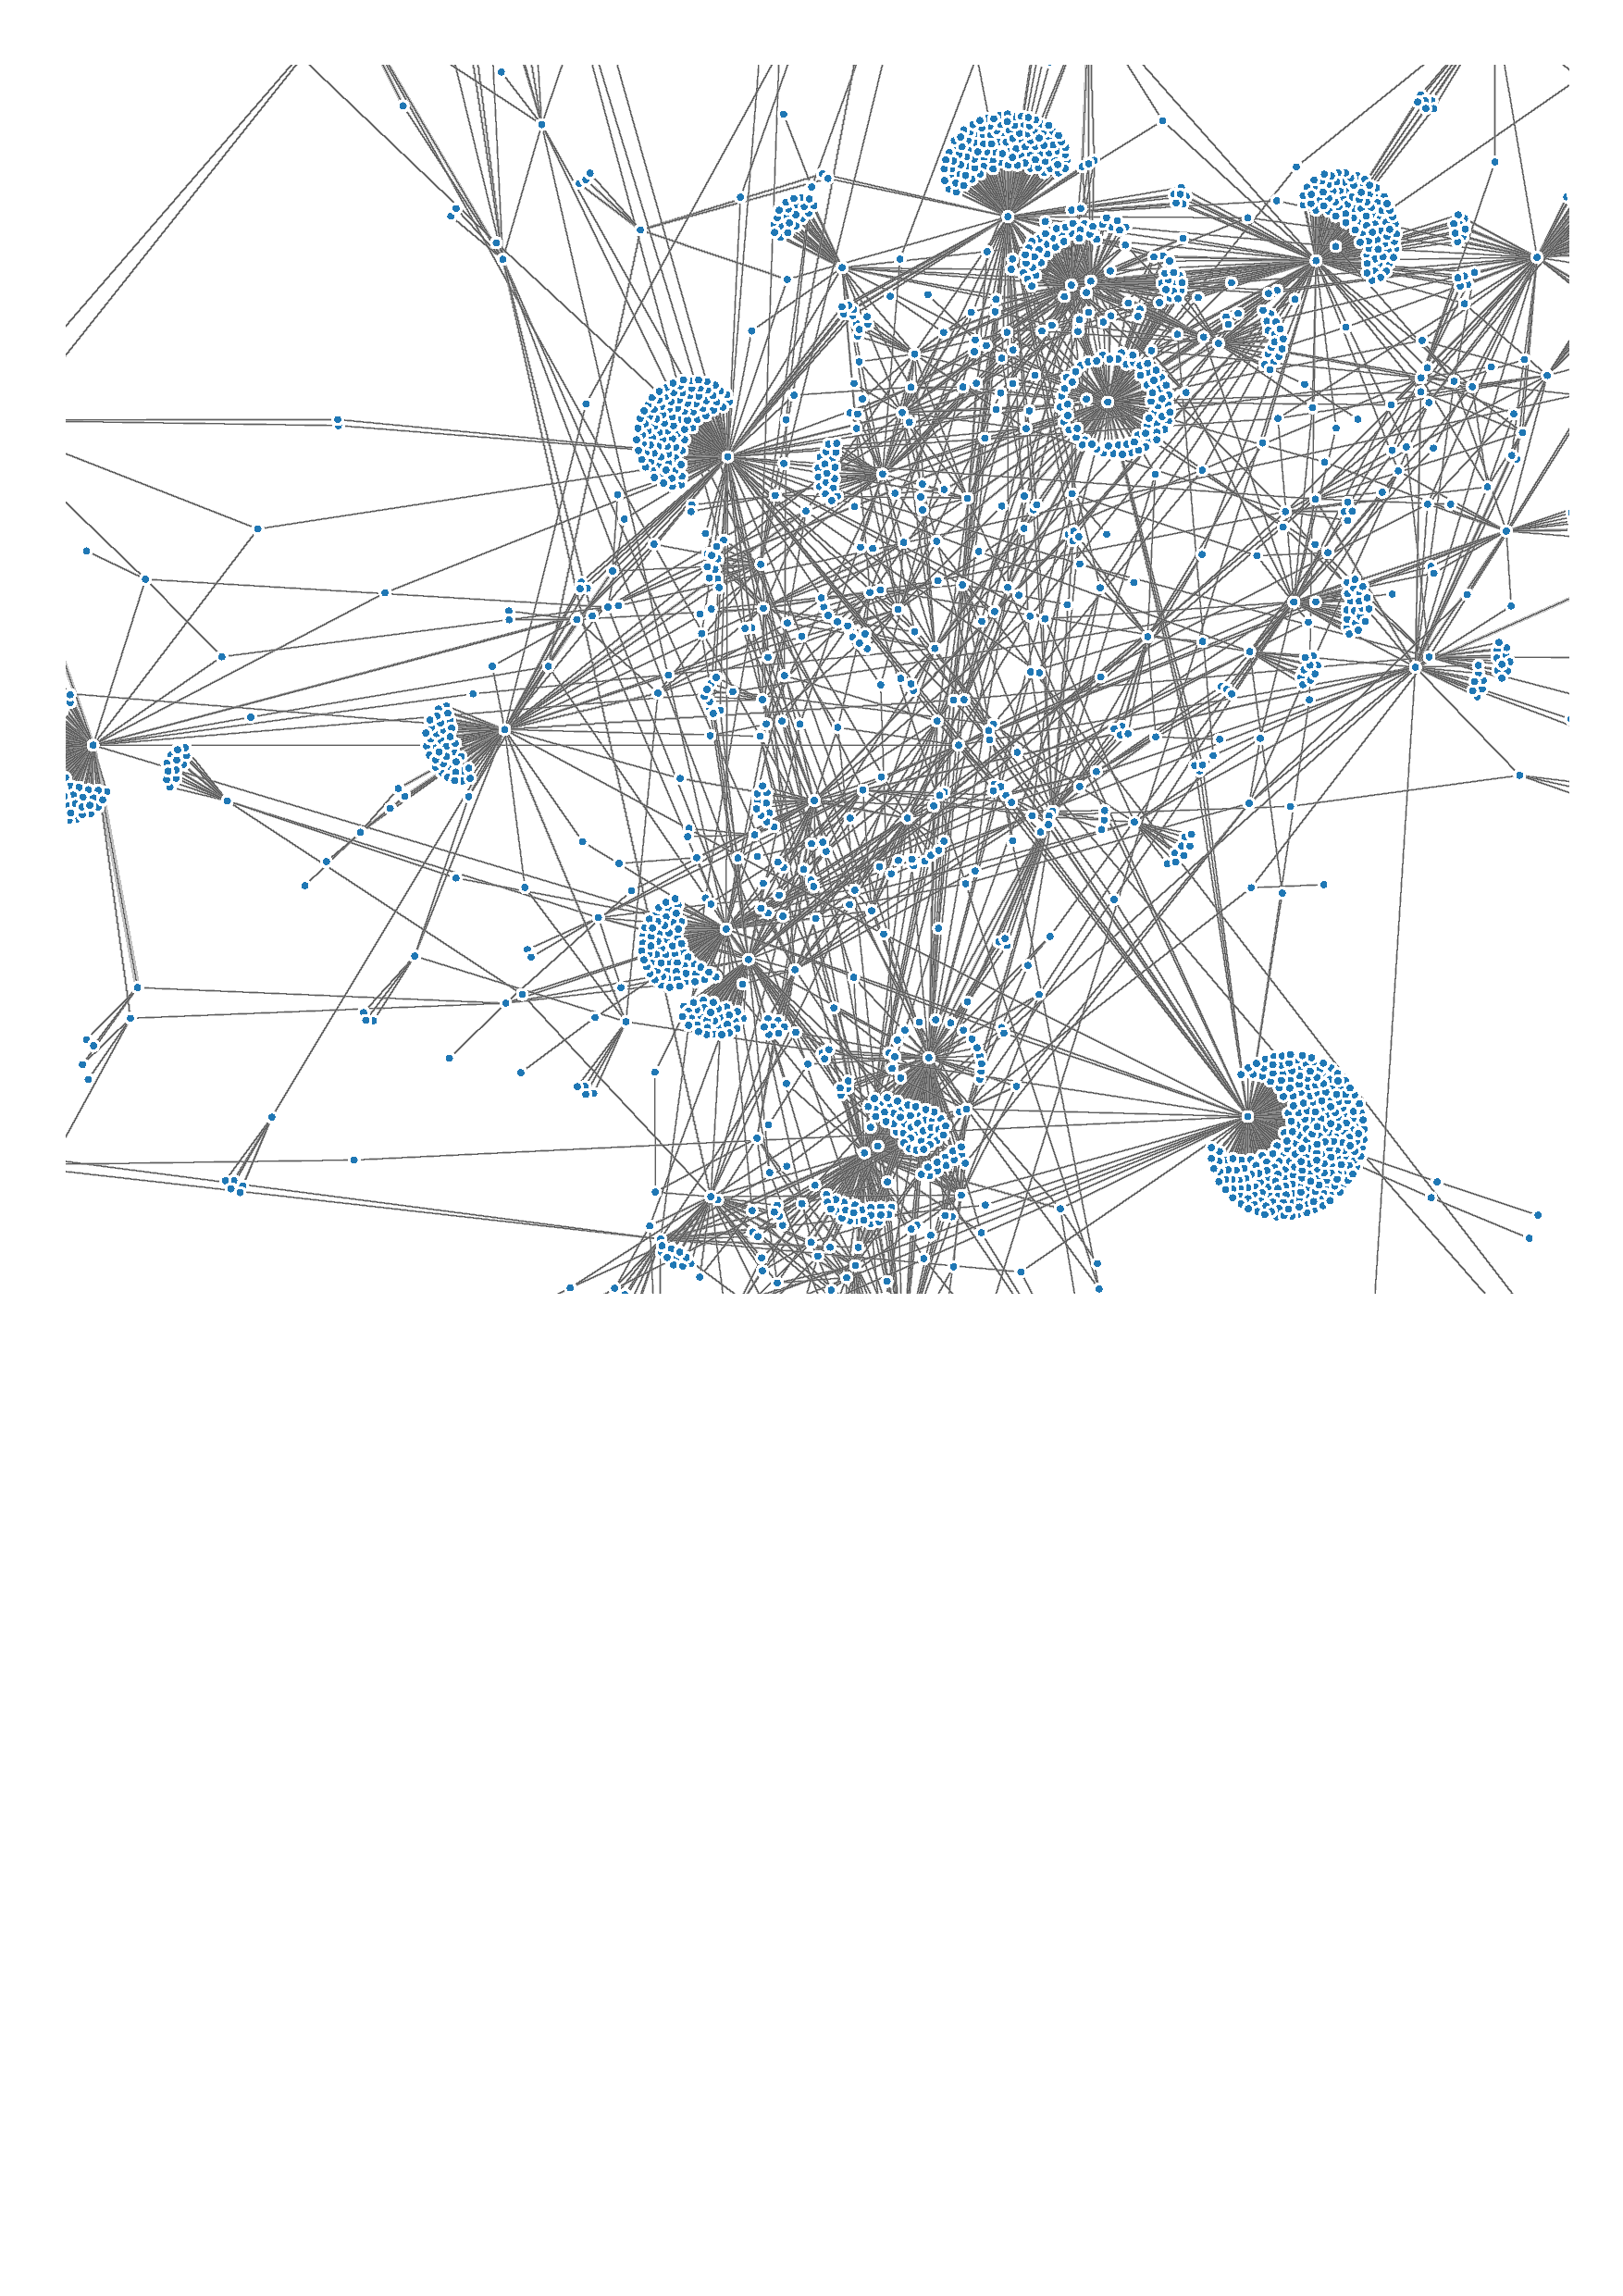
\includegraphics[%
		trim={8cm 32cm 1cm 4cm},% left bottom right top
		clip,%
		width=0.9\textwidth]{network}%
	};%
	\end{tikzpicture}
	\caption{Traditional basic visualisation of a communication graph from 2000 emails using force layout}
	\label{fig:netvis}
\end{figure*}

\section{Interactive Visualisation}
% this section fills second page (inkl mockup)
% describe objectives and what data is available and how that can be used
Systems for document exploration largely vary in what they display and how the user interacts with them, which is already reflected in the way the data is preprocessed or enriched with external sources. 
The design is primarily dictated by the objectives users have.

We distinguish between a bottom-up approach, in which a user initiates an exploration from a specific document or entity, and a top-down approach, in which the system provides an abstract overview of the entire document collection and the user incrementally refines the search narrowing in to just a few documents.
While a bottom-up approach can provide detailed information from the start, it requires a-priori knowledge by the user.
In contrast, the top-down approach can help a user without prior knowledge to get a sense for the data by visualising high level latent structures of the communication network or the topical distribution.

In the scope of this work we primarily consider documents to be emails or data attached to them.
The sender, recipients, time, and content can directly be extracted from the raw data.
We call these -- and results from further processing -- \textit{dimensions} that can be visualised.
From the contents one may infer named entities, topics, embeddings, or salient phases from the content, while the communication network spanned by sender-recipient pairs can be used to detect salient structures and hierarchies.
The temporal information enables the previously mentioned data to be analysed over time to detect evolving or changing patterns.

There are numerous ways to visualise each dimension on its own or as a combination of many.
The user's objective implies which dimension is needed, optional, or irrelevant and also which priority each dimension gets in the visualisation.
From the wide range of possibilities, we strive for a system which helps journalists or investigators to explore a large collection of documents without any prior knowledge about the content and individuals involved.

Thus, we consider the names or email addresses of senders and recipients (from now on \textit{individuals}), the communication network, semantic vector representations of email contents, and as part of an overlay the timestamps of emails.
\Fref{fig:mockup} shows a manually drawn mockup of the system we are working on.


\begin{figure*}
	%	\centering
	\begin{tikzpicture}[]
	\node[draw,anchor=north west,inner sep=1] at (0,0) {%
		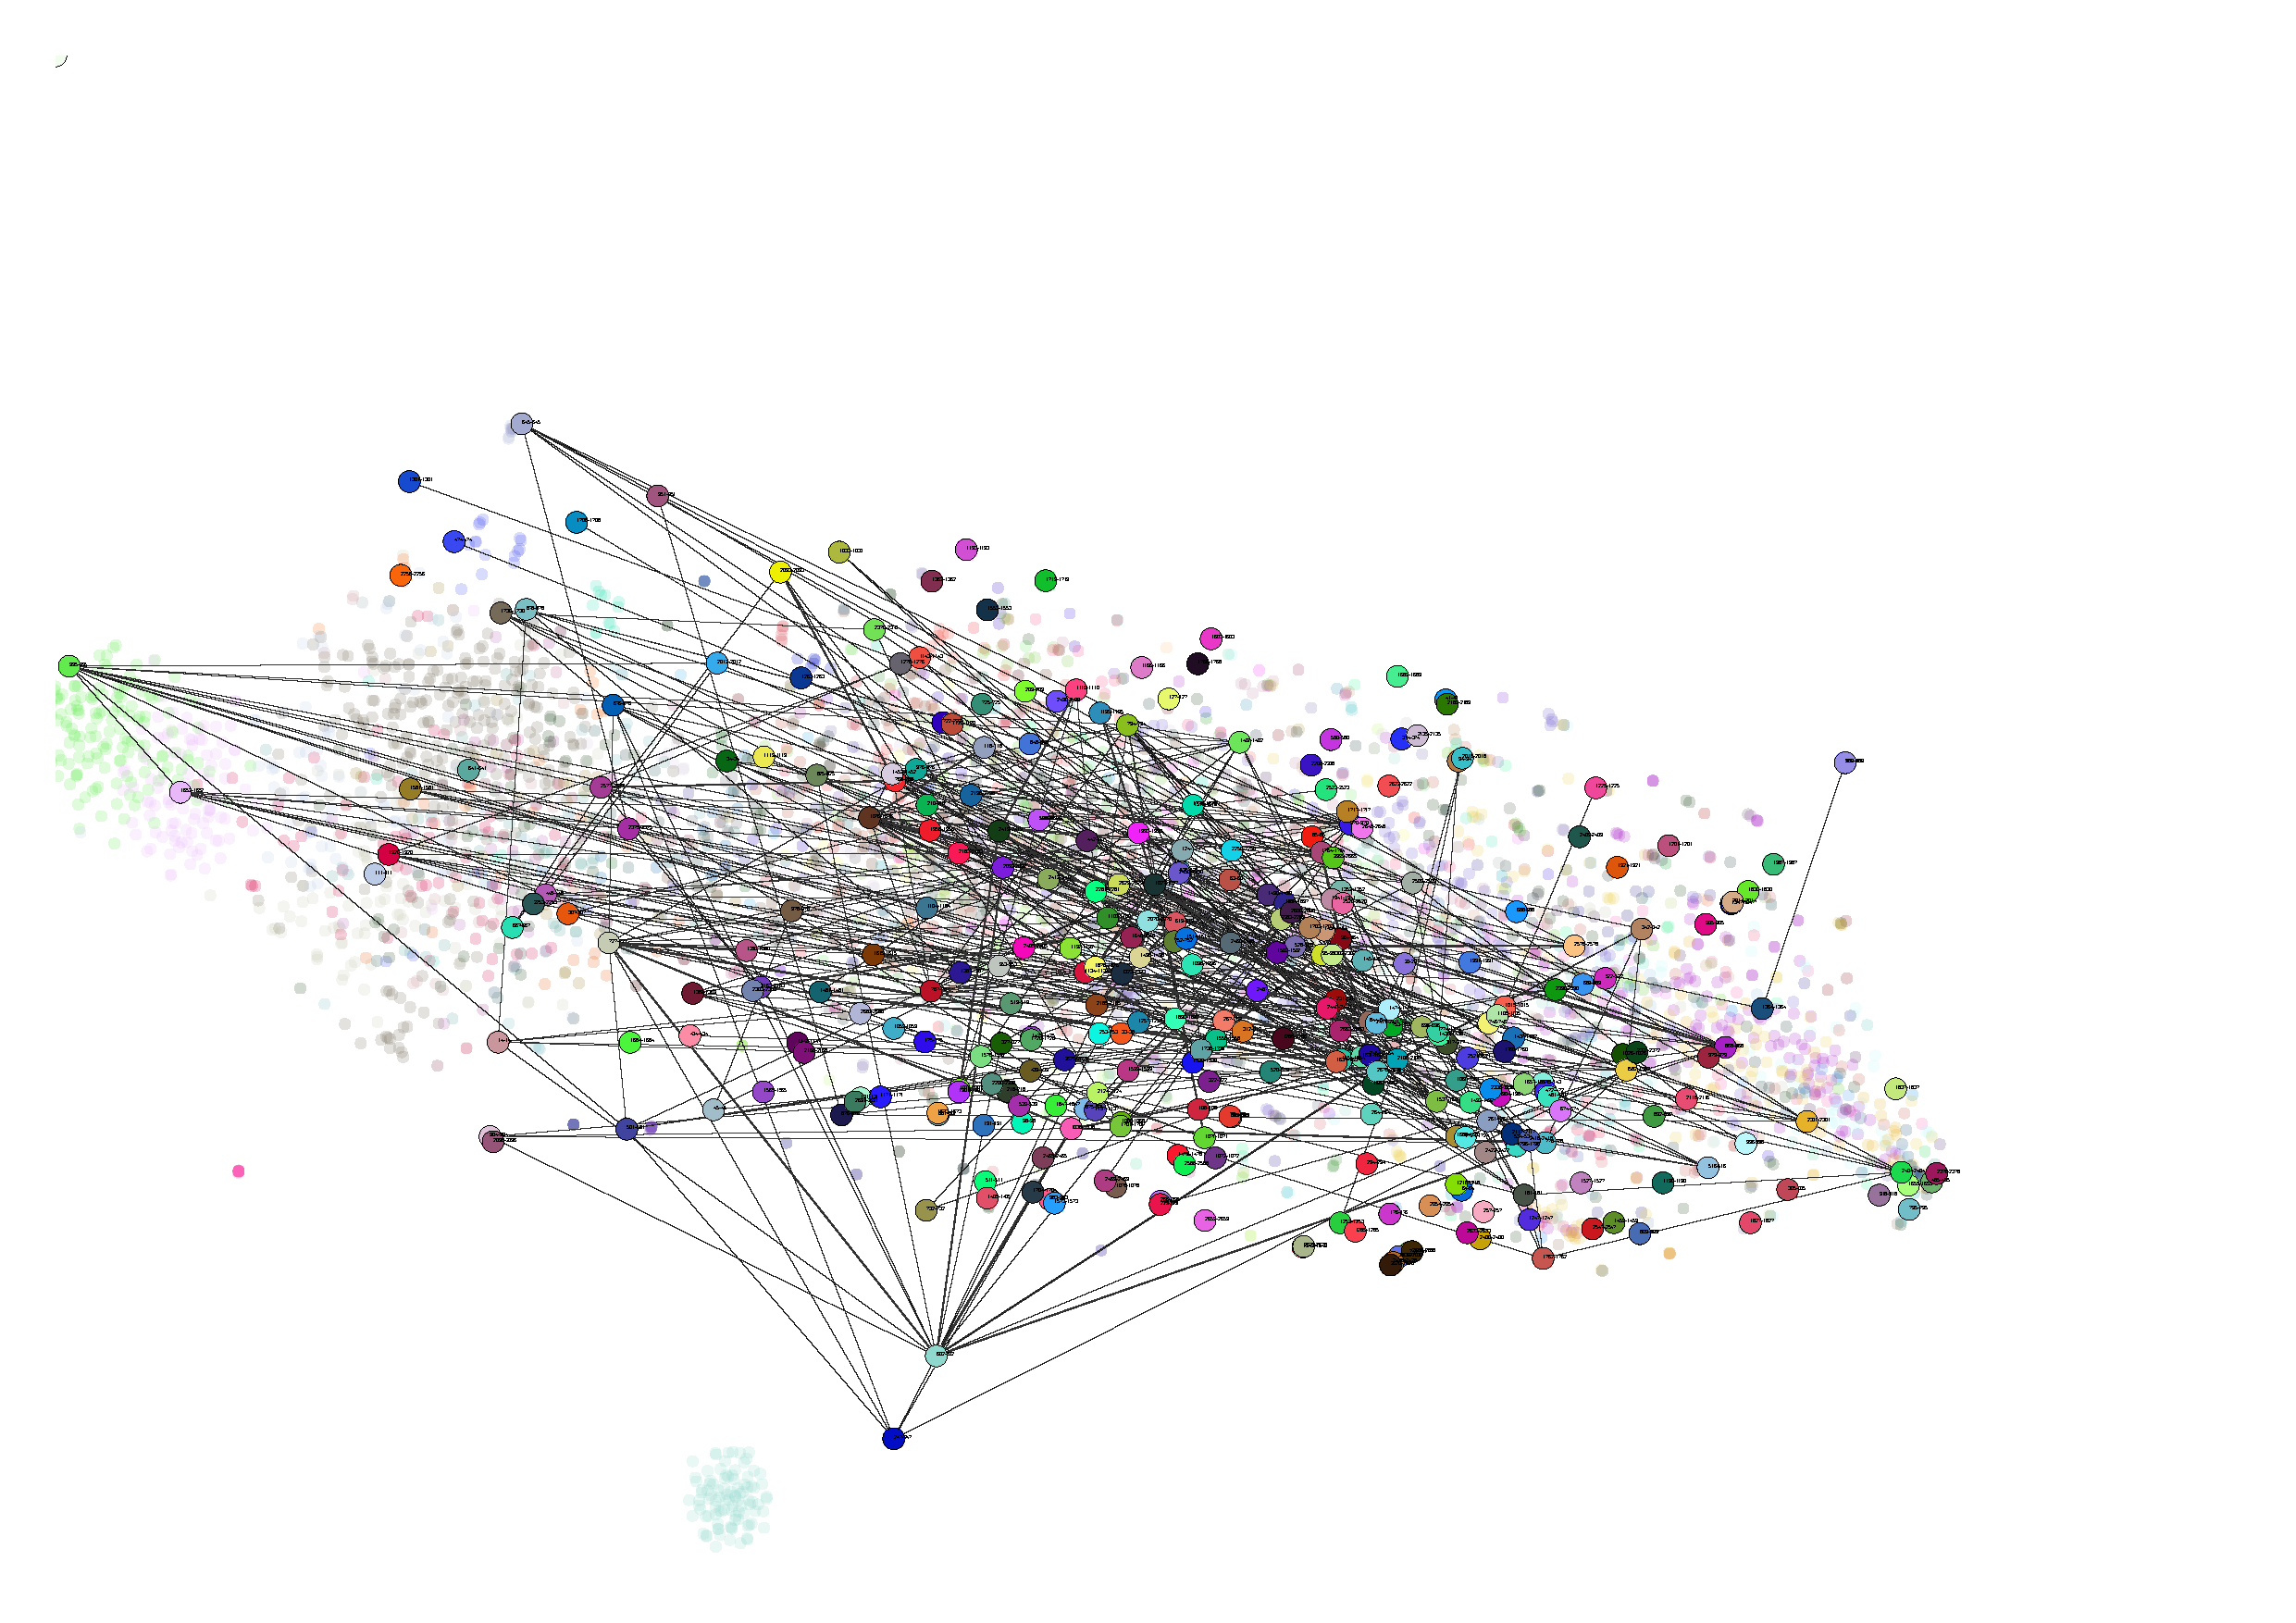
\includegraphics[%
		trim={1cm 13.5cm 20cm 10cm},% left bottom right top
		clip,%
		width=0.9\textwidth]{poc}%
	};%
	\end{tikzpicture}
	\caption{Rendering of the visualisation after initialisation (very early prototype)}
	\label{fig:poc}
\end{figure*}

%We further distinguish between domain oriented and open systems. 
%A domain oriented system may have specific vis, extract, ext data,...


\section{System Architecture}
% fills full page 3 and max the first half of left column page 4
%describe concrete system and outline algorithmic approach
Visualising communication networks in a topic-aware fashion to explore documents and salient structures is not straight forward, as different layout objectives may produce contradicting results.
In this section, we describe algorithmic approaches behind the system we are working on.
For a discussion of engineering aspects on how to store, serve, and render the map-like data, we refer to the Cartograph~stack~\cite{sen2017cartograph}, as we will focus on the process how to extract the information that the map is generated from.
% self citation -> quagga for preprocessing?

As described in the previous section, we visualise the embedded emails as dots in a two-dimensional landscape in which individuals are placed as nodes connected by edges.
By reducing all emails between two individuals into one edge, we reduce the visual complexity of the network, which makes it easier to detect salient structures.
However, that comes with the trade-off, that nodes and edges cannot be perfectly placed in the landscape to cover all semantic aspects of the communication between them, but rather an estimate.

Our proposed algorithm to find a stable network layout has three stages, namely an \textit{(i) initialisation phase} which creates the landscape and roughly places nodes and connections, an \textit{(ii) update phase} which iteratively updates the node placement towards a better fit, and finally a \textit{(iii) post processing phase} where edges become splines to better match the landscape.

%One na\"ive approach to combine a flat visualisation of the document embedding space and communication graph is to assume the embedded emails to be fixed and place the nodes of the graph close to where most emails are projected to.
%This way, many edges may cross each other and communities can't be visually distinguished.
%Furthermore, in case emails of an individual contain two dominant subjects which are far apart in the semantic space, ideal placement of the node becomes ambiguous.

%We assume, that the communication between two individuals 

%optimise towards
%stable balance

\paragraph{Initialising the Landscape.}
First, we need to generate the document landscape.
Therefore, we train document embeddings~\cite{le2014distributed,hu2017} over all emails and use these embeddings to infer high dimensional semantic vector representations for each email.
These vectors are then reduced in dimensionality using t-SNE~\cite{maaten2008visualizing}, which retains possible clustering of emails in the higher dimensional space and can be used to place them onto a two-dimensional map.
The size of a dot printed on the map is determined by the number of recipients of that email.

We also need to initialise the layout of the communication network.
The staring position of a node representing an individual is determined by summing up the two-dimensional vectors of all emails he or she sent or received normalised by the absolute number.
This way, we not only place a node in the semantically relevant region but also implicitly group related individuals into communities as frequent communication biases this normalised sum.
Straight edges are added between the nodes if the respective individuals exchanged emails.
Note, that in the Enron corpus, many edges only represent a small number of emails.
Applying a variable threshold can reduce the computational load in later stages, as these edges will not impact the overall layout very much.
They can be added again as the user requests a detailed visualisation by zooming in or other interactions.

%filter low freq, no influence on layout

Lastly, we apply node2vec~\cite{grover2016node2vec} to the communication graph, as it will be used to measure the neighbourhood similarity between two nodes in later stages of the algorithm.

\paragraph{Adjusting the Network Layout.}
The first stage of our proposed algorithm produces a fixed document landscape and roughly fits the communication network on top. 
We now aim to incrementally adapt the layout of the graph to better reflect salient structures in the network and aligning the edges to the contained emails in the landscape.
Therefore we define a score quantifying how well the current layout fits these objectives:
\begin{equation}
\sum_{n}^{nodes}\left[\sum_{m}^{\substack{emails\\from~n}}\frac{len(E(n, R(m)))}{sim(n, R(m))}\theta+dist(m, E(n,R(m)))\eta\right]
\label{eq:score}
\end{equation}

where $R(m)$ is the recipient of email $m$, $len$ the length of an edge $E$, $sim$ the node2vec based similarity reflecting the neighbourhood affiliation, and $dist$ the shortest distance from the email $m$ to an edge. The parameters $\theta$ and $\eta$ are used to adjust the layout towards a better semantic or structural fit respectively.

%\begin{figure}
%	% alternatively use teaserfigure (manual page 18)
%	% A special kind of figure is used for many two-column conference proceedings. This figure is placed just after the authors, but before the main text. The environment teaserfigure is used for these figures. This environment must be used before \maketitle
%	\dummyfig{0.15}{0.2}{post init example}
%	\dummyfig{0.15}{0.2}{post layout example}
%	%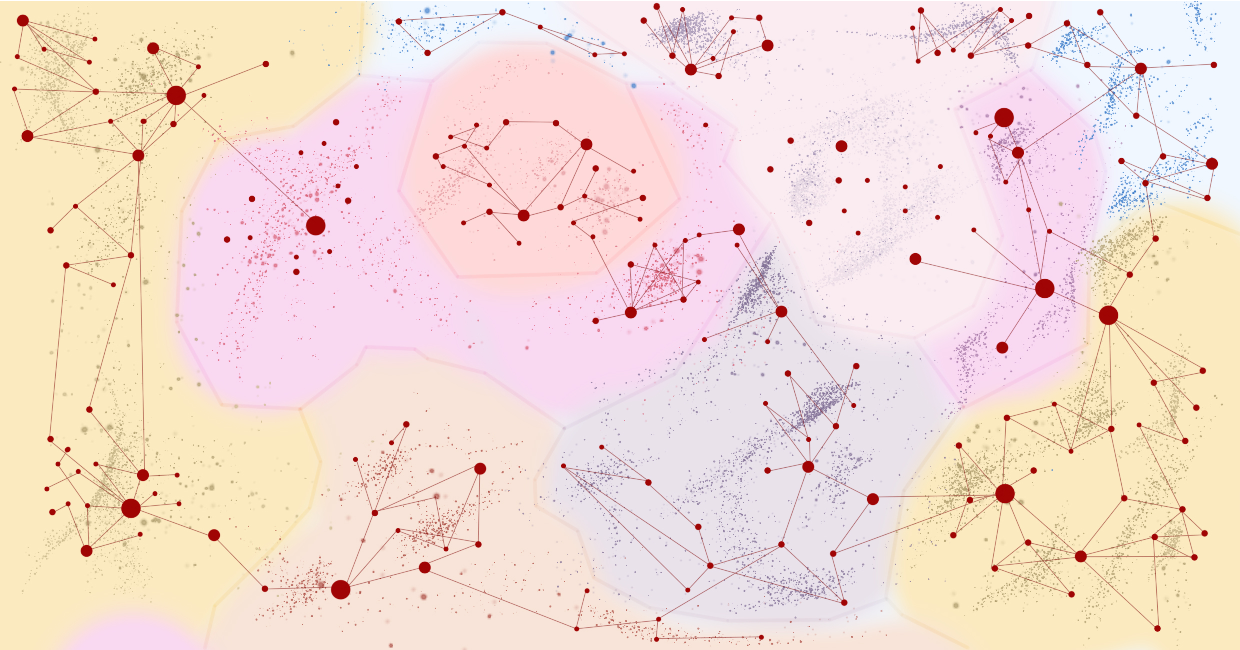
\includegraphics[width=0.9\textwidth]{mockup2}
%	\caption{Schematic example after initialisation (left) and after layout optimisation (right). Nodes and edges of the graph are blue, green dots are embedded emails, dotted lines are email--edge relationships, arrows are update vectors}
%	\label{fig:minisample}
%\end{figure}

%\Fref{fig:minisample} schematically shows a small possible scenario after initialisation.
There, the network layout does not yet reflect our objectives very well as communities are spread apart and mixed.
We incrementally move the nodes towards a stable minimum of \Fref{eq:score}.
The direction 

\paragraph{Post Processing.}
bend and bundle edges, calculate network "topology" (community density as heatmap or topological lines), colour the graph (using topic clustering in case layout isn't close to landscape or community colouring if communities aren't visually close enough -> future research)

%parts of the system: prep, server, frontend
%\begin{itemize}
%\item node2vec
%\item node clustering/communities
%\item doc2vec
%\item tsne for docs in cluster
%\item find stable layout
%\item calculate metric for node importance
%\item calculate metric for salient phrases
%\item use last three for map generation with zoom levels
%\item mapserver, database, leaflet (see cartograph)
%\end{itemize}
%
%describe idea of fully neural approach: feed doc2vec and node2vec to second stage network, use that representation only; discuss outcome (nice because fully semantic and no intervention, bad because outcome unpredictable and potentially visually not practical)

\section{Conclusion and Vision}
\begin{figure*}
	%	\centering
	\begin{tikzpicture}[]
	\node[draw,anchor=north west,inner sep=1] at (0,0) {%
		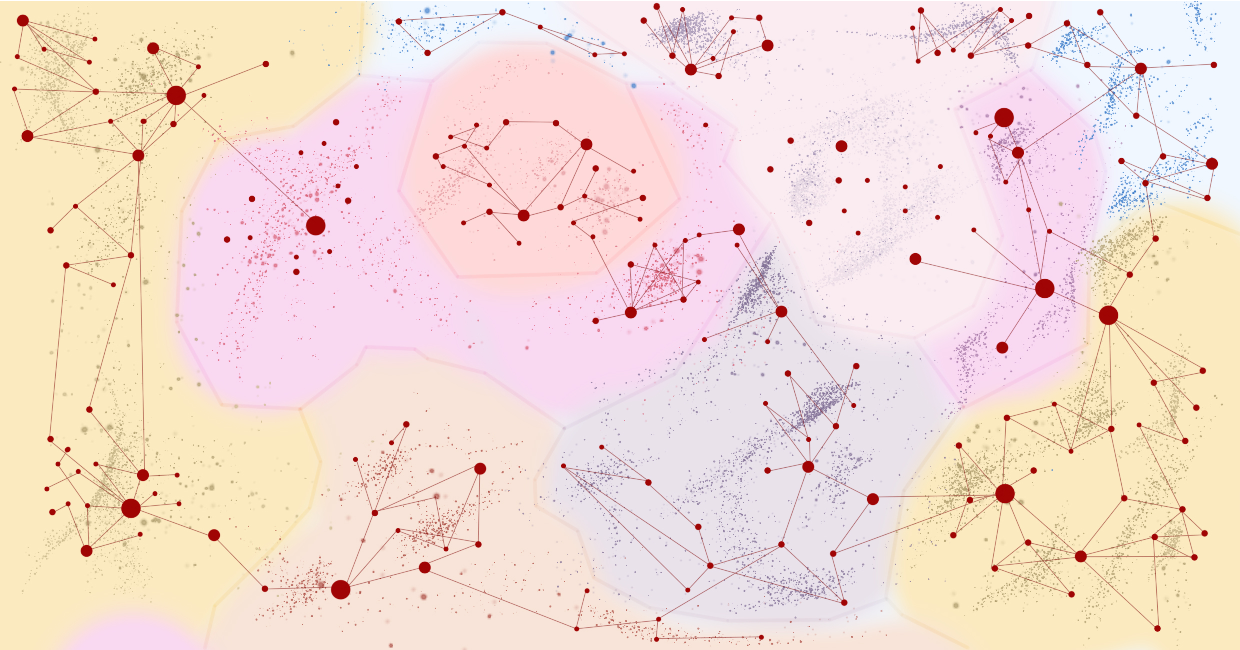
\includegraphics[%
		trim={0 4cm 0 0.5cm},% left bottom right top
		clip,%
		width=0.9\textwidth]{mockup2}%
	};%
	\end{tikzpicture}
	\caption{Semantic landscape of email contents and dominant communication patterns (drawn mockup)}
	\label{fig:mockup}
\end{figure*}
The individuals are represented as nodes positioned such that densely connected communities are visually clustered.
Edges describe the email traffic, where the opacity and thickness is used to indicate the frequency of messages between the nodes they connect.
The semantic representations of emails are used to place dots on a background layer which we call the \textit{document landscape}.
This landscape is used as additional input to the graph layout algorithm, aiming to place a node within corresponding semantic regions.
The colouring of regions in the landscape is derived from densely connected communities in the communication graph.
We select representative words for densely populated areas in the landscape, so that users get a rough idea about subjects in that area.
The aforementioned timestamps of emails can be used to generate a heatmap overlay to show the activity in a certain time interval which is controlled by a slider.

Similar to modern geographical maps, zooming into a region reveals more details.
In our case, less prominent individuals and their connections are shown along with additional salient phrases from the document landscape.
Selecting a node will not only highlight connected edges but may also temporarily show more edges which were previously hidden at that zoom level.
The user will also be able to retrieve documents with the help of a selection rectangle or clicking dots in the document landscape.


% fills left column on page 4, right column mostly references
\begin{itemize}
	\item nice app of big data to find salient communication structures in semantic space
	\item highlight contribution (combine network vis and text vis)
	\item future: implement it, refine algorithm, evaluate usefulness
\end{itemize}

\bibliographystyle{ACM-Reference-Format}
\bibliography{bib} 

\end{document}
